%===========================================================================
\documentclass[uebung]{ETHIDSCprogramming_dpoc}

%\usepackage{german}
%\usepackage[latin1]{inputenc}
%\usepackage{float}
%\usepackage{amsfonts}
%\usepackage{amssymb}
\usepackage{array, longtable}




%---------------------------------------------------------------------------
 \vorlesungstitel{Dynamic Programming and Optimal Control}
 \vorlesungsnummer{151-0563-01}
 \semester{Fall 2011}
 \info{Mohanarajah Gajamohan ({\tt gajan@ethz.ch}), \today}

 \uebungsnummer{2}
 \thema{TBD}

 \ausgabe{Nov 23, 2011}
 %\vorbesprechung{29.\,10.\,03}
 \abgabe{Dec 07, 2011}
 %\nachbesprechung{Nov 5/19, 2008}

 \textbook{BERTSEKAS}

%---------------------------------------------------------------------------

% Some definitions
\newcommand{\field}[1]{\mathbb{#1}}
\newcommand{\R}{\field{R}}

%---------------------------------------------------------------------------

\sloppy
\begin{document}

\maketitle

\begin{center}
\vspace{0.6cm}
\large\textbf{Policy Iteration, Value Iteration and Linear Programming}
\end{center}
\medskip

Consider the task of driving an under powered car up a steep mountain road as shown below. Assume that the car remains on the road at all times.
\begin{figure}[h!]
\begin{center}
    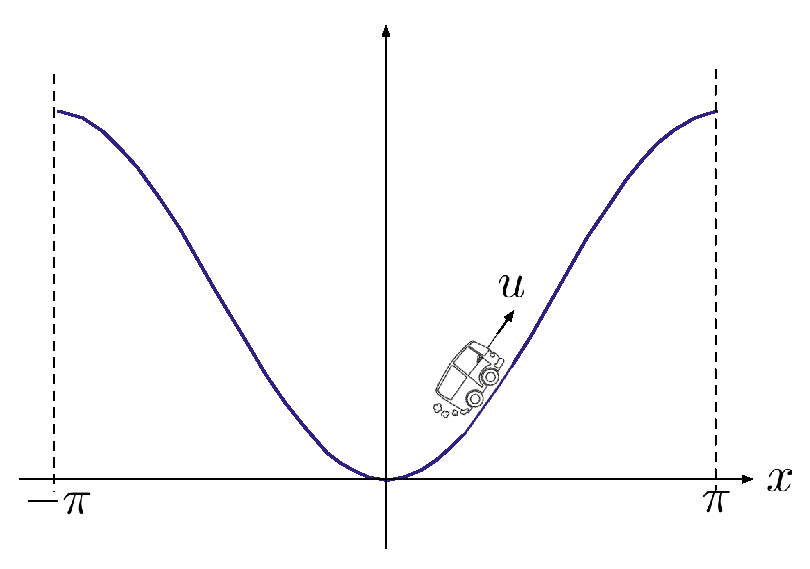
\includegraphics[scale=0.6]{img/mceps.eps}
\end{center}
\end{figure}

The maximum acceleration of the car, $u$, along the road in both directions is limited to $u_{\mathrm{max}}>0$. The discrete time dynamics of the car is given by
\begin{eqnarray}
v_{k+1} &=& v_k + a_x(v_k,x_k,u_k) \Delta t,  \nonumber \\
x_{k+1} &=& x_k + v_k  \Delta t + 0.5 a_x(v_k,x_k,u_k) {\Delta t}^2,  \nonumber
\end{eqnarray}
where $v_k$, $x_k$ are the velocity and position of the car along the horizontal direction ($x$-direction), $\Delta t$ is the discrete time interval, $a_x$ is the acceleration along the horizontal direction is given by,
\begin{equation}
a_x(v_k,x_k,u_k) = -\frac{\sin x_k \cos x_k}{1+\sin^2 x_k} {v_k}^2 -  \frac{\sin x_k}{1+\sin^2 x_k} g -\frac{1}{(1+\sin^2 x_k)^\frac{3}{2}} u_k \nonumber, 
\end{equation}
and $g$ is the gravitational acceleration. 

The goal is find the optimal policy that takes the car to the mountain top, $x\ =\ \pi $ or  $x\ =\ -\pi $, starting from any given postion $x_0 \in (-\pi,\pi)$ and $v_0 \in (-1,1)$ in minimal time (time optimal policy). Three different algorithms are to be implemented to solve this problem:
\begin{itemize}
	\item[(i)] Policy Iteration
	\item[(ii)] Value Iteration: The result of (i) might be used to provide a meaningful stopping criterion for the value iteration algorithm. 
	\item[(iii)] Linear Programming
\end{itemize}

\subsubsection*{Deliverables}
Please hand in by e-mail
\begin{itemize}
\item your implementation of the above three algorithms along with the following function implementation:
 
{\tt [T,Xstar,Ustar,TE] = progEx2Solver(x0, g, opt)} 

\textbf{Input}

\subitem {\tt x0}: vector of initial conditions $[v_0, x_0]^{\mathrm{T}}$
\subitem {\tt g}: gravitational acceleration
\subitem {\tt opt}: algorithm option ({\tt 'valIt', 'polIt', 'linProg'})

\textbf{Output}
\subitem {\tt T}: column vector of time points.
\subitem {\tt Xstar}: optimal-state array. Each row in Xstar corresponds to the state at a time returned in the corresponding row of T.
\subitem {\tt Ustar}: optimal-input array. Each row in Xstar corresponds to the state at a time returned in the corresponding row of T.
\subitem{\tt TE}: The time at which the reaches the top $x\ =\ \pi $ or  $x\ =\ -\pi $
\item surf plot of the cost-to-go values against the states, $v_k$ and $x_k$.
\item in a PDF file, answers to the following question
\begin{enumerate}
\item Physical interpretation of optimal policy
\item Physical interpretation of the discontinuities cost-to-go plots
\end{enumerate}
\end{itemize}
Please include all files into one {\tt zip}-file, which you name {\tt DPOCEx2\_Names.zip}, where {\it Names} is a list of the full names of all students who have worked on the solution.\footnote{Up to three students are allowed to work together on the problem.  They will all receive the same grade.}  
\smallskip 

Send your file to Gajan ({\tt gajan@ethz.ch}) until the due date indicated above.  We will send a confirmation e-mail upon receiving your e-mail.  You are ultimately responsible that we receive your solution in time.


\subsubsection*{Plagiarism}
When handing in any piece of work, the student (or, in case of a group work, each indi-
vidual student) listed as author conrms that the work is original, has been done by the
author(s) independently and that s/he has read and understood the \textit{ETH Citation etiquette}
(http://www.ethz.ch/students/exams/plagiarism s en.pdf ). Each work submitted will be tested
for plagiarism


\end{document}
%===========================================================================
